%gibt an: Papierformat, einseitiger Druck, Schriftgr��e
\documentclass[a4paper,oneside,titlepage,12pt]{article}
%-------------------------------------------------------------------
\usepackage[a4paper, top=2cm, footskip=0pt, headheight=0.8cm, headsep=0.6cm, lmargin=3cm, rmargin=2cm]{geometry}
\usepackage{graphicx}
\usepackage{helvet}
\usepackage{amsmath}
\usepackage{amsthm}
\usepackage{amssymb}
\usepackage{hyperref}
\usepackage[right]{eurosym}
\usepackage[latin1]{inputenc}

%--------------------------------------------------------------------
\renewcommand{\baselinestretch}{1.2}

\begin{document}
%--------------------------------------------------------------------
%Titelseite
\begin{titlepage}
	
\includegraphics{grafiken/HTW-Logo.png}
	%
\includegraphics[width=.3\textwidth]{grafiken/HTW-Logo.png}
	\vspace*{3cm}
	\begin{center}
		\Huge{Benutzerdokumentation\\} \vspace*{1cm}
		\huge{Case-Gruppe 04\\}
		\vspace*{1cm}
		\Large{
			Modul: Software Engineering II\\}
		\vspace*{2cm}
		\normalsize{
			Studiengang Informatik\\
		}
	\end{center}
	\vspace{2cm}
\begin{center}
\large{Sommersemester 2014}
\end{center}
	\vspace*{3cm}



\end{titlepage}

\thispagestyle{empty}\clearpage

%-----------------------------------------------------------------------------------------------------------------------------------
%\rmfamily \pagestyle{fancy} \setcounter{secnumdepth}{4}
\newtheorem{satz}{Satz}
\newtheorem{lemma}[satz]{Lemma}
\newtheorem{folgerung}[satz]{Folgerung}
\theoremstyle{definition}
\newtheorem{definition}[satz]{Definition}
\numberwithin{equation}{section}
\renewcommand{\proofname}{Beweis}

\pagenumbering{roman}\setcounter{page}{3} \tableofcontents
\newcounter{roemisch} \setcounter{roemisch}{\value{page}}
\clearpage

\setcounter{page}{2} \pagenumbering{arabic}

\section{Einleitung}
Das entwickelte Software-System dient zur Verwaltung von Beleggruppendaten und
besteht aus genau 2 Programmen. Eines f�r die Studenten zum Anmelden und
Verwalten ihrer eigenen Gruppe und zum anderen ein Programm f�r den Dozenten,
welcher haupts�chlich administrative Funktionen besitzt.\\
Die vorliegende Dokumentation soll den Benutzern die grundlegenden Funktionen
beider Programme verst�ndlich darstellen.

\section{Voraussetzungen}
\begin{itemize}
  \item Microsoft .Net Framework Version 4.5 muss installiert sein
  \item nur im HTW-internen Netzwerk ausf�hrbar, au�erhalb �ber VPN
  \begin{itemize}
    \item[] 
\includegraphics{grafiken/Verbindungsfehler.png}\\
  \end{itemize}
\end{itemize}

\section{Erstanmeldung}
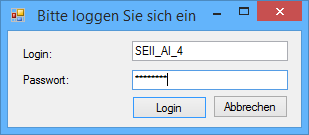
\includegraphics{grafiken/Student_ELogin.png}\\
\\Beim Programm-Start wird der sich einloggende Student aufgefordert die
Gruppenkennung und das Gruppenpasswort einzugeben.
Falls es sich hierbei um eine Erstanmeldung handelt, m�ssen nun die vom Dozenten
bekanntgegebenen Erstlogin-Daten eingegeben werden.
\\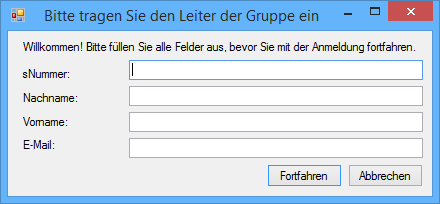
\includegraphics{grafiken/Student_Login_Erstlogin.png}\\
\\Als n�chstes m�ssen die Daten eines Studenten der Gruppe eingegeben werden.
Dieser Student wird provisorisch als Gruppenleiter festgelegt und im
n�chsten Fenster angezeigt. Dies ist jedoch nicht verbindlich, da die
Verantwortlichkeiten innerhalb der Gruppe noch nachtr�glich ge�ndert werden
k�nnen. 
\\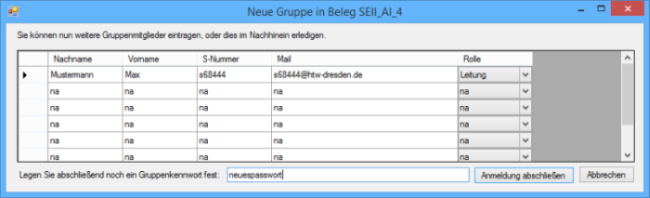
\includegraphics{grafiken/Student_Login_Erstlogin_abschliessen.png}\\
\\Im n�chsten Schritt muss ein Gruppenpasswort festgelegt werden, welches
unten in das Textfeld eingegeben werden muss und mit welchem sich die Gruppe zuk�nftig
anmelden kann. Die Gruppe bekommt abschlie�end die Gruppenkennung angezeigt,
welche den Benutzernamen bei allen zuk�nftigen Anmeldungen darstellt. Die
Gruppe sollte sich also diese Gruppenkennung und das vorher selbst gew�hlte
Passwort unbedingt merken!\\
\\
\includegraphics{grafiken/Student_Login_Erstlogin_abschliessen_wirklich.png}\\
Im n�chsten Fenster k�nnen die restlichen Mitglieder eingetragen werden und ein
Thema aus dem Themen-Pool (Combobox unten) ausgew�hlt werden.
\\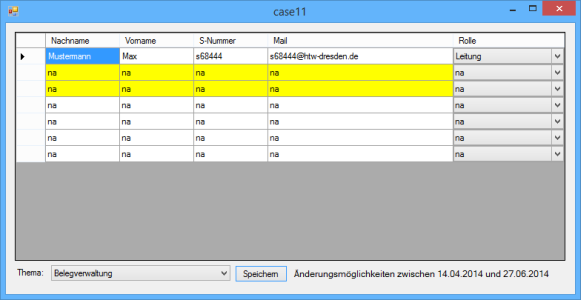
\includegraphics{grafiken/Student_Zusammenfassung.png}
\\Zum Schluss k�nnen alle Gruppendaten gespeichert werden.



\section{Anmeldung}
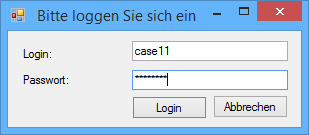
\includegraphics{grafiken/Student_Login.png}\\
Der Anmeldebildschirm ist der selbe wie bei der Erstanmeldung, jedoch wird bei
der normalen Anmeldung nicht der von dem Dozenten bekanntgegebenen Login
eingegeben, sondern die case-Gruppe als Benutzernamen und das selbst gew�hlte
Passwort. Falls die eingegebene Kombination aus case-Gruppe (Benutzername) und
dem Passwort richtig ist, erscheint die �bersicht der Gruppe mit den
Studenten-Daten.\\
\\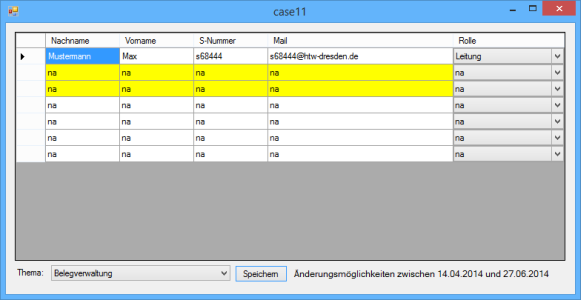
\includegraphics{grafiken/Student_Zusammenfassung.png}\\
\\Solange der Bearbetungszeitraum nicht �berschritten ist, k�nnen hier
beliebeige �nderungen vorgenommen werden.

\end{document}